\section{Methodology}

\subsection{Device Characteristics}
It is important to know the characteristics of the devices being used for computation. The architecture of a device can determine its suitability for sequential work, or the degree of its parallel effectiveness. OpenCL provides built-in methods to view the characteristics of its devices.

\begin{Cpp}
clGetDeviceInfo(clGetDeviceIDs()[0], cl_device_info.###) // Intel Device
clGetDeviceInfo(clGetDeviceIDs()[1], cl_device_info.###) // NVIDIA Device
// where ### is the device parameter in question

\end{Cpp}

%can maybe make this a distinct section rather

\subsection{Kernel Performance on CPU vs GPU}
OpenCL kernels perform a function and can be assigned to an OpenCL device for execution. Kernels can be executed sequentially, in parallel on a single device, or on multiple devices. This section focuses on analysing the performance of a sum kernel running on the provided Intel CPU versus the provided NVIDIA GPU. The implementation requires writing a sum kernel, shown below:
\begin{Cpp}
kernel void sum(global float *a, global float *b, global float *c){
  int gid = get_global_id(0);
  c[gid] = a[gid] + b[gid];}
\end{Cpp}

An OpenCL context is created for each device:
\begin{Cpp}
nvidia_platform = pyopencl.get_platforms()[0]
nvidia_devices = nvidia_platform.get_devices()
nvidia_context = pyopencl.Context(devices=nvidia_devices)
intel_platform = pyopencl.get_platforms()[1]
intel_devices = intel_platform.get_devices()
intel_context = pyopencl.Context(devices=intel_devices)
\end{Cpp}


The sum kernel is built for each device:
\begin{Cpp}
nvidia_program_source = pyopencl.Program(nvidia_context,program_source)
nvidia_program = nvidia_program_source.build()
intel_program_source = pyopencl.Program(intel_context,program_source)
intel_program = intel_program_source.build()
\end{Cpp}


CPU-only program:
\begin{OpenCL}
# Code provided by the 2017 EEE4084F OpenCL Workshop
# Memory buffers are created
a_intel_buffer = pyopencl.Buffer(intel_context,
                                 flags=pyopencl.mem_flags.READ_ONLY, 
                                 size=a.nbytes)
b_intel_buffer = pyopencl.Buffer(intel_context, 
                                 flags=pyopencl.mem_flags.READ_ONLY, 
                                 size=b.nbytes)
c_intel_buffer = pyopencl.Buffer(intel_context, 
                                 flags=pyopencl.mem_flags.WRITE_ONLY, 
                                 size=c.nbytes)
# Command Queue
intel_queue = pyopencl.CommandQueue(intel_context)
def run_cpu_program():
    #copying data onto CPU
    pyopencl.enqueue_copy(intel_queue,
                          src=a,
                          dest=a_intel_buffer)
    pyopencl.enqueue_copy(intel_queue,
                          src=b,
                          dest=b_intel_buffer)
    
    #running program
    kernel_arguments = (a_intel_buffer,b_intel_buffer,c_intel_buffer) 
    intel_program.sum(intel_queue,
                       a.shape, #global size
                       None, #local size
                       *kernel_arguments)

    #copying data off CPU
    copy_off_event = pyopencl.enqueue_copy(intel_queue,
                                           src=c_intel_buffer,
                                           dest=c)
    copy_off_event.wait()
\end{OpenCL}
GPU-only program:
\begin{OpenCL}
# Code provided by the 2017 EEE4084F OpenCL Workshop
# Memory buffers are created
a_nvidia_buffer = pyopencl.Buffer(nvidia_context,
                                 flags=pyopencl.mem_flags.READ_ONLY, 
                                 size=a.nbytes)
b_nvidia_buffer = pyopencl.Buffer(nvidia_context, 
                                 flags=pyopencl.mem_flags.READ_ONLY, 
                                 size=b.nbytes)
c_nvidia_buffer = pyopencl.Buffer(nvidia_context, 
                                 flags=pyopencl.mem_flags.WRITE_ONLY, 
                                 size=c.nbytes)
# Command Queue
nvidia_queue = pyopencl.CommandQueue(nvidia_context)
def run_gpu_program():
    #copying data onto CPU
    pyopencl.enqueue_copy(nvidia_queue,
                          src=a,
                          dest=a_nvidia_buffer)
    pyopencl.enqueue_copy(nvidia_queue,
                          src=b,
                          dest=b_nvidia_buffer)
    
    #running program
    kernel_arguments = (a_nvidia_buffer,b_nvidia_buffer,c_nvidia_buffer) 
    nvidia_program.sum(nvidia_queue,
                       a.shape, #global size
                       None, #local size
                       *kernel_arguments)

    #copying data off CPU
    copy_off_event = pyopencl.enqueue_copy(nvidia_queue,
                                           src=c_nvidia_buffer,
                                           dest=c)
    copy_off_event.wait()
\end{OpenCL}


\subsection{Counting Factors}
A more complex task to allocate to the devices is generating a matrix of random integers, and calculating the number of factors each element has. This required the implementation of a new kernel, shown below.

\begin{Cpp}
kernel void checkfactors(global int *X, global int *c, int row_length){
  int gid = row_length*get_global_id(0) + get_global_id(1);
  int num = 1;
  int max = X[gid];
  if(X[gid] > 100)
    max = 100;
  else
    max = X[gid];
  for(int i = 2; i <= max; i++){
      if(X[gid]%i == 0)
          num++;}
  c[gid] = num;}
\end{Cpp}

More than one operation is conducted for every element in the matrix, and this should lead to a different set of results when compared to the sum kernel mentioned previously. For simplicity it was decided that square matrices should be used for testing, but rectangular matrices can be used with only slight alteration to the code. To initialise the program, the size of the matrix is specified, and filled with random integers. An empty matrix is initialised, and this is where the output of the function will be written.

\begin{lstlisting}[language=Python]
N = M = numpy.int32(1e4)
X = numpy.random.randint(100,size=(N,M)).astype(numpy.int32)
c = numpy.empty_like(X)
\end{lstlisting}

The program is built in much the same way as the sum kernel was, for both the CPU and GPU, although one less memory buffer is required and the parameters taken by the kernel function are slightly different.

%\begin{figure}
%\centering
%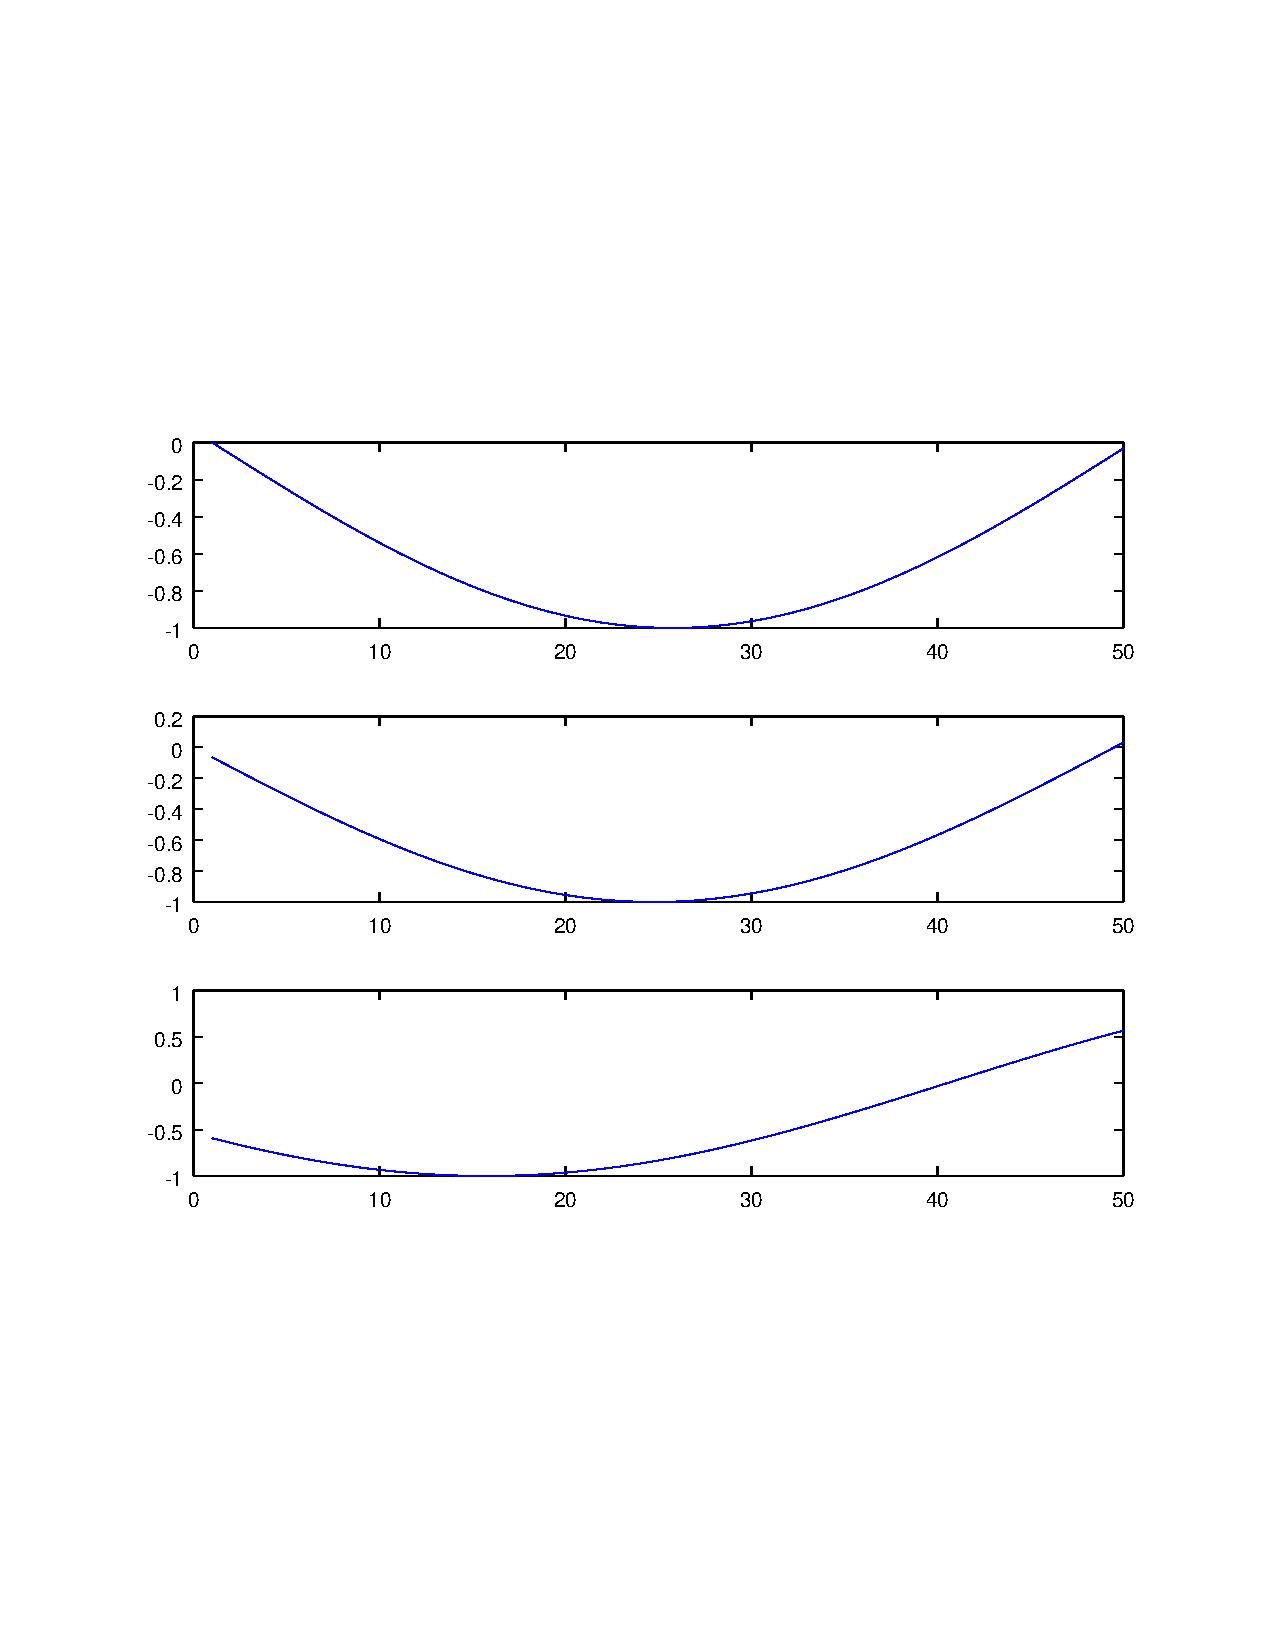
\includegraphics[scale=0.4]{Figures/lofreq}
%\caption{Different windows of the same signal}
%\label{fig:windowslo100}
%
%
%
%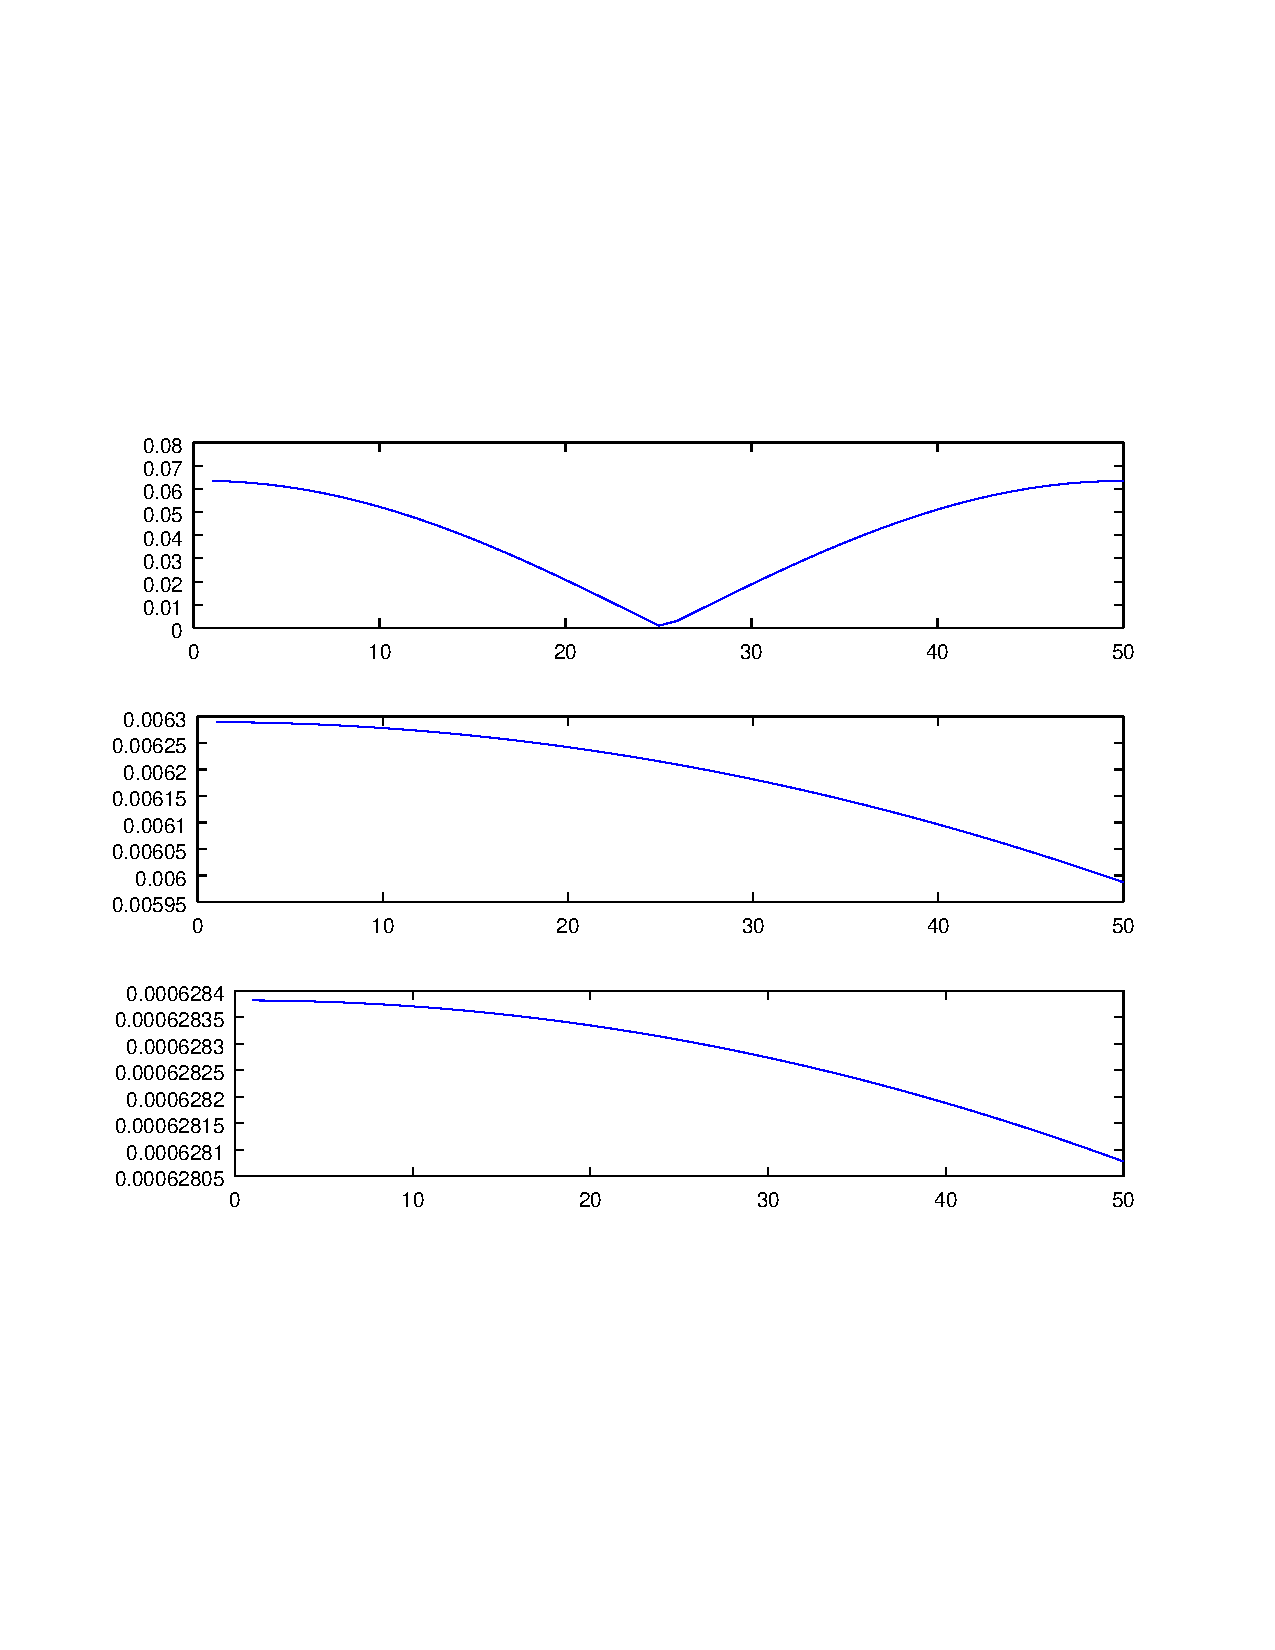
\includegraphics[scale=0.4]{Figures/absvals}
%\caption{Absolute differences between a signal and shifted counterpart, according to sample rate}
%\label{fig:absvals}
%\end{figure}
